\documentclass{sig-alternate}


\usepackage{enumitem}
\usepackage{framed}
%\usepackage[11pt]{moresize}
\usepackage{cprotect}
\usepackage{enumitem}
\usepackage{listings}
\usepackage{amstext}
\usepackage{amstext}
\usepackage{pdfpages}
\usepackage{alltt}
\usepackage{epstopdf}
\usepackage{xspace,colortbl}
\usepackage[USenglish]{babel}
\usepackage{multirow}
\usepackage[hyphens]{url}
\usepackage{subfigure}
\usepackage{graphicx}%%
\usepackage{amssymb}
\usepackage{fmtcount}
\usepackage{amsfonts}
\usepackage{xspace}
\usepackage{amsmath}
\usepackage{multirow}
\usepackage[mathscr]{eucal}
%\usepackage{psfrag}
\usepackage{colortbl}

\usepackage{amsmath,amssymb}
\usepackage[linesnumbered, ruled,vlined]{algorithm2e}

\usepackage{caption}
\usepackage{graphicx}

\usepackage{bm}
\usepackage[nospace]{cite}
\usepackage{csquotes}
\usepackage{enumitem}
\usepackage{times}

\usepackage{courier}

\lstset{basicstyle=\scriptsize\ttfamily,breaklines=true}
\lstset{framextopmargin=50pt}

\usepackage{cleveref}

\usepackage{balance}

%\linespread{0.99}

\makeatletter
\def\@copyrightspace{\relax}
\makeatother


\DeclareMathOperator*{\argmin}{arg\,min}
\DeclareMathOperator*{\argmax}{arg\,max}
\newcommand*{\QEDB}{\ensuremath{\square}}%



\begin{document}

%\setlength{\belowdisplayskip}{3pt} \setlength{\belowdisplayshortskip}{3pt}
%\setlength{\abovedisplayskip}{3pt} \setlength{\abovedisplayshortskip}{3pt}
%\setlength{\belowcaptionskip}{-10pt}
%\selectfont

\newtheorem{theorem}{Theorem}
\newtheorem{example}{Example}
\newtheorem{definition}{Definition}
\newtheorem{problem}{Problem}
\newtheorem{property}{Property}
\newtheorem{proposition}{Proposition}
\newtheorem{lemma}{Lemma}
\newtheorem{corollary}{Corollary}

\newcommand{\detectlib}{\texttt{IsoDetect}\xspace}
\newcommand{\company}{\texttt{Company X}\xspace}
\newcommand{\cond}{\textrm{pred}\xspace}
\newcommand{\dataset}{data set\xspace}
\newcommand{\datasets}{data sets\xspace}
\newcommand{\spview}{\textsf{SPView}\xspace}
\newcommand{\fjview}{\textsf{FJView}\xspace}
\newcommand{\aggview}{\textsf{AggView}\xspace}
\newcommand{\hashfunc}[1]{\textsf{hash}(#1)\xspace}
\newcommand{\hashop}{\textsf{hash}\xspace}
\newcommand{\nsc}{\textsf{NormalizedSC}\xspace}
\newcommand{\rsc}{\textsf{RawSC}\xspace}

\newcommand{\avgfunc}{\ensuremath{\texttt{avg} }\xspace}
\newcommand{\maxfunc}{\ensuremath{\texttt{max} }\xspace}
\newcommand{\minfunc}{\ensuremath{\texttt{min} }\xspace}
\newcommand{\histfunc}{\ensuremath{\texttt{histogram\_numeric} }\xspace}
\newcommand{\countfunc}{\ensuremath{\texttt{count}}\xspace}
\newcommand{\sumfunc}{\ensuremath{\texttt{sum} }\xspace}
\newcommand{\varfunc}{\ensuremath{\texttt{var} }\xspace}
\newcommand{\stdfunc}{\ensuremath{\texttt{std} }\xspace}
\newcommand{\covfunc}{\ensuremath{\texttt{cov} }\xspace}
\newcommand{\corrfunc}{\ensuremath{\texttt{corr} }\xspace}
\newcommand{\medfunc}{\ensuremath{\texttt{median} }\xspace}
\newcommand{\percfunc}{\ensuremath{\texttt{percentile} }\xspace}
\newcommand{\havingfunc}{\ensuremath{\texttt{HAVING} }\xspace}
\newcommand{\selectfunc}{\ensuremath{\texttt{select} }\xspace}
\newcommand{\ratio}{\ensuremath{\rho }\xspace}


\newcommand{\insertion}{\ensuremath{\texttt{INSERT} }\xspace}
\newcommand{\update}{\ensuremath{\texttt{UPDATE} }\xspace}
\newcommand{\delete}{\ensuremath{\texttt{DELETE} }\xspace}

\newcommand{\sysfull}{AlphaClean\xspace}
\newcommand{\sys}{AlphaClean\xspace}
\newcommand{\sysnospace}{AlphaClean}


\newcommand{\tbl}[1]{\textsf{#1}\xspace}
\newcommand{\field}[1]{\textsf{#1}\xspace}
\newcommand{\cost}{\textrm{cost}\xspace}
\newcommand{\ans}{\textsf{ans}\xspace}
\newcommand{\dans}{\Delta\textsf{ans}\xspace}
\newcommand{\cqp}{correction query processing\xspace}
\newcommand{\Cqp}{Correction query processing\xspace}

\newcommand{\reminder}[1]{{{\textcolor{magenta}{\{\{\bf #1\}\}}}\xspace}}
\newcommand{\ewu}[1]{{{\textcolor{blue}{\{\{\bf ewu:\} #1\}}}\xspace}}
\newcommand{\mps}[1]{{{\textcolor{red}{\{\{\bf meelap:\} #1\}}}\xspace}}
\newcommand{\stitle}[1]{\smallskip\noindent\textbf{#1: }}


\definecolor{light-gray}{gray}{0.95}
\definecolor{mid-gray}{gray}{0.85}
\definecolor{green}{RGB}{0,176,80}
\definecolor{darkred}{rgb}{0.7,0.25,0.25}
\definecolor{darkgreen}{rgb}{0.15,0.55,0.15}
\definecolor{darkblue}{rgb}{0.1,0.1,0.5}
\definecolor{orange}{RGB}{237,125,49}
\definecolor{blue}{RGB}{68,114,196}
\definecolor{pop}{RGB}{0,21,245}

\newcommand{\white}[1]{{\textcolor{white}{#1}\xspace}}
\newcommand{\blue}[1]{{\textcolor{blue}{{\bf #1}}\xspace}}
\newcommand{\orange}[1]{{\textcolor{orange}{{\bf #1}}\xspace}}
\newcommand{\pop}[1]{{\textcolor{pop}{{\textit{\textbf{#1}}}}\xspace}}
\newcommand{\red}[1]{\textcolor{red}{#1}}
\newcommand{\green}[1]{\textcolor{green}{#1}}
\newcommand{\gray}[1]{\textcolor{light-gray}{#1}}




\newcommand{\specialcell}[2][c]{%
  \begin{tabular}[#1]{@{}c@{}}#2\end{tabular}}

\def\ojoin{\setbox0=\hbox{$\bowtie$}%
  \rule[-.02ex]{.25em}{.4pt}\llap{\rule[\ht0]{.25em}{.4pt}}}
\def\leftouterjoin{\mathbin{\ojoin\mkern-5.8mu\bowtie}}
\def\rightouterjoin{\mathbin{\bowtie\mkern-5.8mu\ojoin}}
\def\fullouterjoin{\mathbin{\ojoin\mkern-5.8mu\bowtie\mkern-5.8mu\ojoin}}

%\setlength{\belowcaptionskip}{-10pt}

%\newcommand{\reminder}[1] {}
\pagestyle{plain}

%\input{coverletter.tex}

\title{\sys: Iterative Learning Search for Data Cleaning}


\numberofauthors{1}
\author{ Sanjay Krishnan$\,^{*}$, Michael J. Franklin$\,^{*\dag}$, Ken Goldberg$\,^{*}$, Eugene Wu{$\,^{\dag\dag}$}  \\
\affaddr{ $^*$UC Berkeley, ~~ $^\dag$University of Chicago, ~~ $^{\dag\dag}$Columbia University} \\
\affaddr{ \{sanjaykrishnan, franklin, goldberg\}@berkeley.edu ~~ ewu@cs.columbia.edu}\\
\affaddr{}
}

%\fontsize{9pt}{11pt}
%\selectfont


\maketitle

\begin{abstract}
Data cleaning is widely reported to be one of the most human-intensive steps in the analysis process.
We explore to what extent such transformation rules can be learned through a process of automatic trial-and-error on a dataset.
The system simulates different sequences of data transformations and scores the result according to a user-specified data quality objective function.
Inspired by recent work in AI, such as playing Go~\cite{silver2016mastering} and in Atari video games~\cite{mnih2015human}, we propose an iteratively learning search model that applies the trial-and-error procedure to small blocks of data and incrementally learns a model to prune the trials.
This basic algorithm has a number of important advantages: (1) it is highly expressive as it can model a wide range of data cleaning formalisms from integrity constraints to quantitative data cleaning in the same framework, (2) it exhibits parallelism not only over the data but also over search algorithm, and (3) the result of the algorithm is not only a cleaned database instance but transformations that can be applied to future data.
We present a system called \sys, which is built around this algorithm.
\sys additionally provides an API for specifying special-case optimizations. 
In our experiments, we find that \sys achieves parity with state-of-the-art specialized constraint, statistical, and quantitative data cleaning systems in terms of accuracy.
On two datasets considered in prior data cleaning work of Flight arrival times and a Physician registry, \sys achieves a similar precision and recall to a recently proposed (2017) Denial Constraint system called HoloClean. 
Similarly, we applied \sys to numerical outlier problems and compared to the Minimum Covariance Determinant (MCD) algorithm, which is the basis of another recent system (2017) called Macrobase.
Outliers removed by \sys  improved the accuracy of a downstream predictive models more significantly than MCD (5\% prediction accuracy improvement on the US Census Dataset) and a (4\% on an EEG dataset). 
Finally, we present initial results demonstrating the scaling properties of \sys where parallelism and caching can reduce search time by nearly two orders of magnitude.
\end{abstract}


%\pagenumbering{gobble}


\section{Introduction}\label{intro}\sloppy
It is widely known that data cleaning is one of the most time-consuming steps of the data analysis process~\cite{nytimes}, and
designing algorithms and systems to automate or partially automate data cleaning continues to be an active area of research~\cite{DBLP:conf/sigmod/ChuIKW16}.
Automation in data cleaning is challenging because real-world data is highly variable. 
A single data set can have many different types of data corruption such as statistical outliers, constraint violations, and duplicates.
Once an error is detected, there is a further question of how to repair this error, which often depends on how the data will be used in the future.

This variability creates a tension between the needs of the data scientist and the designer of the data cleaning framework.
While the data scientist might desire a single cleaning framework that addresses all of her data errors and repair operations, from an algorithmic perspective, it is far more efficient to consider more restricted models.
Data cleaning tools are often highly optimized for particular problems  (e.g., see statistical outliers~\cite{hellerstein2008quantitative}, enforcing logical constraints~\cite{DBLP:conf/sigmod/ChuIKW16}, entity resolution~\cite{DBLP:journals/pvldb/KopckeTR10}). 
Consequently, a recent survey of industry suggests that data cleaning pipelines are often a patchwork of custom scripts and multiple specialized systems~\cite{krishnan2016hilda}.
The overhead to setup, learn, and manage multiple cleaning systems can easily outweigh their benefits.
Some data scientists eschew automated tools altogether and simply write data cleaning programs from scratch.
The customized programming approach quickly becomes difficult to mantain and interpret; especially for users without data engineering expertise~\cite{sculley2014machine}.

We believe that a single cleaning system that exposes a sufficiently flexible interface can address the above challenges as long as the runtime can be made comparable to existing alternatives.  
To this, we turn to the modern AI and planning literature, which has produced exciting results such as AlphaGo~\cite{silver2016mastering} that were previously considered not possible.    This work shows that a combination of machine learning and massively parallelized search can effectively optimize highly complex objective functions.
Our main observation is that data cleaning is very similar to AI planning problems~\cite{russell1995modern}.
In planning, the system is given a state space and actions that transition between states, and incrementally generates a sequence of actions one move at a time (a plan) that will ultimately maximize a quality function. The classic application is a computer chess program that must plan a sequence of chess moves that change the state of the board in order to maximize the likelihood of a checkmate. Likewise, in data cleaning, one is given a dirty relation and a way to measure data quality (e.g., number of integrity constraints violated), and the data cleaning problem is to find a sequence of modifications to the relation that maximize the data quality metric.

Most non-trivial planning problems are very hard without good search heuristics.
Advances in machine learning have made it possible to replace hand-crafted heuristics with automatically learned pruning functions that estimate the expected quality of candidate plans. AlphaGo learned pruning heuristics using a neural network trained on data generated through self-play~\cite{silver2016mastering}. 
The key insight is that expertly written heuristics can be replaced with data-driven models, which makes the techniques applicable to a diverse set of applications.   
This insight is highly relevant to data cleaning, where datasets tend to have structure amenable to learning heuristics adaptively.
Data errors are often systematic where they are correlated with with certain attributes and values in the dataset~\cite{rekatsinas2017holoclean,DBLP:journals/pvldb/KrishnanWWFG16}.
Consequently, as more data is cleaned, we can better identify common patterns to prioritize the search on future data.

\sys is a new data cleaning system that is designed around a search-based architecture. It takes as input a {\it quality function} that models the data quality of a relation as a real-value between $[0,1]$ and a {\it language} of parameterized data cleaning operators, and outputs a sequence of data cleaning transformations (a cleaning program) from the language that seeks to maximize the quality function.This API imposes minimal restrictions on the quality function, giving it tremendous flexibility in terms of the data errors that it can express.   As a comparison, the recent Holoclean~\cite{holoclean} is similar in that it provides a rich interface to specify denial constraints and lookup tables, and integrates them within a probabilistic model to more accurately resolve constraint violations.  In contrast, \sys's quality function is a UDF that can express {\it arbitrary combinations} of denial constraints {\it as well as} statistical, quantitative, text formatting, and other classes of data errors.  For instance, \Cref{s:expquant} shows how \sys can perform cleaning for machine learning applications by embedding machine learning training and evaluation within the quality function, while \Cref{s:expterror} combines entity resolution, outlier cleaning, and functional dependency violations within the same function.  

\sys uses a best-first search that greedily appends data transformations to the set of best candidate programs seen so far, and adopts parallelization and pruning ideas from the search-based planning literature~\cite{silver2016mastering}.  This can be viewed as a generalization of recent search-based text extraction systems~\cite{jin2017foofah} to a wider range of error measures and optimizations.    In contrast to traditional planning, where the search state (e.g., chess board) is compact and largely trivial to parallelize in a distributed setting, the data cleaning search state is the size of the input dataset and introduces a trade-off between communication costs to share intermediate state and the degree of parallelism possible.  We develop a gather-scatter style method to parallelize \sys in a distributed context. 

To further accelerate its runtime, \sys can also encode problem-specific optimizations as search pruning rules (e.g., disallowed transformation sequences) or modifications to the data representation (e.g., clustering similar records).  We find that many optimizations in existing cleaning systems may be cast as search pruning rules.
More powerfully, \sys can adaptively learn pruning rules to avoid unprofitable search branches during the search process. 
While AlphaGo used a deep neural network and massive amounts of training data to model the heurisitic, our experiments show that a simple logistic regression classifier requires far fewer training examples that can be gathered during the search process and can reduce runtime by multiple orders of magnitude on our experiments. 


It is natural to expect that such a general formulation must sacrifice cleaning accuracy, runtime performance, or both.  Our primary technical contribution is to develop optimizations to provide evidence that neither need be sacrificed\footnote{It is important to acknowledge that \sys loses many of the provable guarantees provided by specialized systems based on logical constraints, and is in some sense, best-effort.  }
Across 8 real-world datasets used in prior data cleaning literature, we show that \sys matches or exceeds the cleaning accuracy, and exhibits competitive runtimes, as compared to state-of-the-art approaches that are specialized to a specific error domain (constraint, statistical, or quantitative errors).  On a mixed error dataset that requires three specialized cleaning systems, we show that \sys has higher precision and recall (\ewu{NUMBERS}) than running the three specialized systems is sequence, generates the cleaning program in \ewu{XXX$\times$} less time.

We believe that unifying disparate data cleaning problems within a single, compact\footnote{The core search and optimization code is $<200$LOC in Python.} framework offers many unique benefits and directions for new data cleaning applications.  These include:

%\begin{itemize}[leftmargin=*, topsep=0mm, itemsep=0mm]
\stitle{Optimization} Existing cleaning pipelines must combine disparate cleaning solutions and manage glue code to transfer data between systems.  However, data transfer can be a non-trivial portion of the total cleaning cost and recent work~\cite{palkar2017weld} has shown that a common runtime can avoid data movement and improve runtimes by up to $30\times$.  Unifying data cleaning within a single search-based framework avoids such overheads and offers optimization opportunities such as parallelization and shared computation between the different error classes.

 \stitle{Generalization and Robustness} In contrast to existing cleaning systems, that output a cleaning relation, \sys outputs a composable cleaning program that is both simpler to understand because it groups common fixes together, and can be applied to new data.  In addition, the cleaning program allows us to analyze cleaning systems for overfitting.  We indeed find that the complexity of the quality function and cleaning language can lead to overfitting, and believe this is the case for any data cleaning system.  We also show that simple changes to the quality function can act as regularization terms to control the degree of overfitting.

 \stitle{Software Engineering} Eschewing multiple cleaning systems simplifies software engineering, and lets users focus on expressing their application's notion of data quality.  Users do not need to write and manage glue code; do not need to manage ETL between systems; and do not need to learn system specific abstractions, languages, and assumptions.  All of these are arguably intangible, but critical friction points in the highly iterative cleaning process.  

 \stitle{New Cleaning Applications} We currently support a programmatic interface using simple Python library, however we envision that a single API makes it possible to support an ecosystem of domain-specific cleaning specification libraries.  For instance,  interactive visualization interfaces akin to~\cite{trifacta,kandel2011wrangler,DBLP:journals/pvldb/0002M13,wu2012demonstration} can directly translate user interactions into a wide range of cleaning constraints.   This can enable an entire population of non-technical domain experts to participate in the data cleaning process.

\smallskip
To summarize, \sys highlights an approach to data cleaning where users articulate high level cleaning goals, and the system automatically proposes an interpretable cleaning program.  It is a step towards a unified framework for automatic data cleaning systems, similar in spirit to the relational model, which combined transaction, analytic, graph, machine learning, and other data-intensive applications under a unified specification, optimization, and execution framework.









% * single library/language with the same abstraction is important (software engineering)
%   * no more glue code -- talk about weld, etc.  
%   * no ETL between systems
%   * no leraning new abstractions
%   * new languages to specify constraints and quality goals.  some are languages, some are APis, some are systems
%   * engineering: systems like llunatic, need to satisfy postgres schema to get started
% 
% * different
%   * application driven cleaning by embedding downstream app into the quality function
%   * new apps
%     * viz stuff needs a single api
%     * mixed datasets -- numeric and relational data
%     * many interfaces to compose and create quality functions and languages
% 
% * holoclean
%   * lets them express denial constraints and use a knowledge base to decide how to resolve violations
%   * we suppor denial constraints, as well as numeric errors, text extraction errors, and arbitrary formulations of teh quality measure.  
% 
% 
% * unification -->
%   * reduces engineering to implement cleaning system
%   * joint optimization if overlapping in 
% * generalize to new data 
%   * overfitting
% * parallelize opportunities












\if{0}
Data cleaning usually involves tedious manual specification of transformation rules.
For example, a data scientist might write a rule that maps every record with a \textsf{country} attribute ``United States'' to ``United States of America''.
These collections of rules quickly grow in size, and if they are developed in an ad-hoc way, they can be brittle and hard to maintain~\cite{krishnan2016hilda}.
Overly specific rules may not apply to future data, and overly general rules, might introduce unwanted side-effects.
Designing accurate transformation rules is a painstaking process, which is widely reported to be one of the most effort-intensive steps in data science~\cite{nytimes}.

We explore to what extent such transformation rules can be learned through a process of automatic trial-and-error on a dataset.
The system simulates different sequences of data transformations and scores the result according to a user-specified data quality objective function.
On its own, this is an inefficient way to search to search the set of transformation rules.
However, we can leverage Machine Learning to learn a strong pruning heuristic incrementally.
Transformations are often parametrized by literal values from the database (e.g., find string X and replace with string Y).
If we clean data in small partitioned blocks, we can incrementally build a classifier that infers common patterns in these literals, such as whether the strings tend to be similar or tend to be different or the attributes that are likely to be touched.
For example, consider the problem above where a data scientist is resolving inconsistencies in a \textsf{country} attribute to satisfy an integrity constraint.
As we iterate through the distinct \textsf{country} values and simulate possible replacement values, it might become clear that the source string have to be close to the target strings in string similarity, i.e., ``United States'' is more likely to be replaced by ``United States of America'' than ``Zimbabwe''.
Learning such a relationship automatically avoids hand coded heuristics which have to consider the complex relationship between how the analyst describes data quality and how exactly the transformations are defined.

This basic algorithm, optimizing a sequence of black-box transformations over a black-box data quality function, has a number of important advantages: (1) it is highly expressive as it can model a wide range of data cleaning formalisms from integrity constraints to quantitative data cleaning in the same framework, (2) it is relatively easy to parallelize the search, and (3) the result of the algorithm is not only a cleaned database instance but transformations that can be applied to future data.
This formalism casts data cleaning as a planning problem; analogous to the algorithms used AI, Robotic Planning, and Control.
Similar to the way one plans out a sequence of chess moves in AI to gain a strategic board position, we can think of data cleaning as planning out a sequence of data transformations to maximize the score on a data quality function.
And as in chess, where one cannot perfectly anticipate the opposing player's moves, in data cleaning we may not have a strong \emph{a priori} model of how a user-defined transformation rule modifies the data.
As a result, the algorithm and search heuristics cannot make strong assumptions about the anticipated structure of any search instance.
This sort of an approach is increasingly attractive because recent results in AI demonstrate scaling these search problems to  high branching-factor domains even when few assumptions are made.
Recent algorithms have been shown to match or exceed human performance in domains such as Go~\cite{silver2016mastering} and in Atari video games~\cite{mnih2015human}.
As in many classical data cleaning problems, an optimal solution to AI search problems is very hard to discover, but pragmatically leverage distributed computing and pruning rules learned from data can tractably find acceptable solutions.

We use this algorithm as a starting point for a new data cleaning system called \sys.
We designed an API that takes classical data cleaning problem specifications, such as integrity constraints, gold-standard manually cleaned data, and statistical models, and translates those specifications into an iterative learning search problem. 
Of course, we often need special-case optimizations that prune unproductive search branches to make the runtime more competitive with special case systems.
We provide a model where pruning rules are specified as regular expressions over a formal language of transformations and can be static (i.e., fixed before execution) and dynamic (i.e., inferred from properties of the dirty database instance).
The search algorithm we use is a memory-bounded best-first search which maintains the subset of the search frontier that can fit in memory. 
This algorithm can be parallelized, distributed, and can cache repeated computations.
\fi



\if{0}


view data cleaning from a planning~\cite{} and optimization perspective, and show evidence that a simple, general approach to this problem can provide the user with considerable flexibility in terms of cleaning data with different classes of errors, controlling the allowable operations, and customizing the system to new types of data errors.



Ideally, the majority of the data cleaning process should reside in a single system with a  \emph{declarative} interface, wherein the analyst specifies a high-level data model (e.g., constraints the data should satisfy) and a system automatically generates the pipeline to enforce the model.
The idea of declarative data cleaning is not new~\cite{rahm2000data}, but such approaches have classically been restricted to data models specified in subsets of first-order logic and only recently have considered extensions better handle uncertain numerical data~\cite{prokoshyna2015combining}.
The prevailing wisdom is that there is an inherent tradeoff between the expressiveness of the data model and the efficiency of the (approximate) solution algorithm---limited models allow the system designer to exploit specific algorithmic structures.


However, two recent trends, namely, the success of model-free learning in AI and the availability commodity cloud computing encourage us to reconsider this algorithmic philosophy.
Recent progress in planning problems such as AlphaGo~\cite{silver2016mastering} and automatically playing Atari video games~\cite{mnih2015human} have shown that a prudent combination of Machine Learning and distributed search can approximately optimize very complex black-box objective functions.
The intriguing aspect of these results is that the same algorithm, called Deep Q Reinforcement Learning, that learns to play an Atari game~\cite{mnih2015human} can be used on a very different problem, such as training a robot~\cite{gu2017deep}.
The underlying optimization algorithm encodes few specifics about the objective or structure of the domain  and pragmatically finds a reasonable local optimum.
The optimization algorithm is general enough to support a very wide class of problems--at the cost of additional computational resources since it is unaware of instance-specific structure.

\fi

\section{Problem Definition}
First, we overview the basic formalism of \sys and present its relationship to related work.

\subsection{Data Transformations}
We focus on data transformations that concern a single relational table. 
Let $R$ be a relation over a set of attributes $A$, and let $\mathcal{R}$ denote the set of all possible relations over $A$.
Let $r.a$ be the attribute value of $a \in A$ for row $r \in R$.
$T(R): \mathcal{R} \mapsto \mathcal{R}$ is a data transformation that maps an input relation instance $R \in \mathcal{R}$ to a new (possibly cleaner) instance $R' \in \mathcal{R}$ that adheres to the same schema.  For instance, ``replace all \texttt{city} attribute values equal to {\it San Francis} with {\it SF}'' may be one data transformation, while ``delete the $10^{th}$ record'' may be another.   Data transformations can be composed using the binary operator $\circ$:
\[
(T_i \circ T_j)(R) =  T_i(T_j(R))
\]
The composition of one or more data transformations is called a {\it cleaning program} $p$.   

In practice, users will specify {\it transformation templates} $T(R, [\theta_1,\cdots,\theta_k])$, and every assignment to the parameters represents one possible transformation.  
\begin{example}\label{ex1}
The following relation contains two attributes \textsf{city\_name} and \textsf{city\_code}.  Suppose there is a one-to-one relationship between the two attributes. In this case, the relation is inconsistent with respect to the relationship and contains errors highlighted in \red{red}.

  \begin{table}[ht!]
  \centering
  \label{my-label}
  \begin{tabular}{|l|l|l|}
  \hline
  \rowcolor[HTML]{000000} 
  & \white{city\_name}            & \white{city\_code}   \\ \hline
  1 & San Francisco                    & SF                                  \\ \hline
  2& \red{\textbf{New York}}           & NY                                  \\ \hline
  3 & New York City                    & \red{\textbf{NYC}} \\ \hline
  4 & \red{\textbf{San Francisc}}      & SF                                  \\ \hline
  5 & San Jose                         & SJ                                  \\ \hline
  6 & San Mateo                        & SM                                  \\ \hline
  7 & New York City                    & NY                                  \\ \hline
  \end{tabular}
  \end{table}

The following transformation template uses three parameters: \texttt{attr} specifies an attribute, \texttt{srcstr} specifies a source string, and \texttt{targetstr} specifies a target string.   
\[
\textsf{find\_replace}(\text{srcstr}, \text{targetstr}, \text{attr})
\]
Given an input relation, the template finds all \texttt{attr} values equal to \texttt{srcstr} and replaces those cells with \texttt{targetstr}. 
For instance, \texttt{find\_replace(``NYC'', ``NY'', ``city\_code'')} defines a data transformation that fixes the error in the second attribute.
\end{example}

Let $\Sigma$ be a set of distinct data transformations $\{T_1,\cdots,T_N\}$, and
$\Sigma^*$ be the set of all finite compositions of $\Sigma$, i.e., $T_i\circ T_j$.
A formal language $L$ over $\Sigma$ is a subset of $\Sigma^*$.
A program $p$ is valid if it is an element of $L$.

\begin{example}\label{ex2}
  Continuing \Cref{ex1}, $\Sigma$ is defined as all possible parameterizations of \texttt{find\_replace}.  Since many possible possible parameterizations are non-sensical (e.g., the source string does not exist in the relation), we may bound $\Sigma$ to only source and target strings present in each attribute's instance domain (a standard assumption in other work as well~\cite{DBLP:series/synthesis/2012Fan}).  In this case, there are $61$ possible data transformations, and $\Sigma^*$ defines any finite composition of these $61$ transformations.  The language $L$ can be further restricted to compositions of up to $k$ data transformations.  
\end{example}

Finally, let $Q(R): \mathcal{R} \mapsto [0,1]$ be a quality function where $1$ implies that the instance $R$ is clean.
In other words, $Q$ scores each possible result of applying a program $p \in \mathcal{L}$ to an initial dirty table $R_{dirty}$.
There are two special cases that we also consider that give us more information. 
We define two sub-classes of quality functions: row-separable and cell-separable quality functions.
The former expresses the overall quality based on row-wise quality function $q(r): R \mapsto [0,1]$ where $1$ implies that the record is clean:
\[Q(R) \propto \sum_{r \in R} q(r)\]
\noindent Similarly, a cell-separable quality function can be expressed based on a cell-wise quality function $q(r, a): (R\times A) \mapsto [0,1]$:
\[Q(R) \propto \sum_{r \in R} \sum_{a \in A} q(r,a)\]
These special cases are important because they can define hints on what types of transformations are irrelevant.
For example, if we have a cell-separable quality function, then we know we can restrict the language of transformations to only those that modify erroneous cells and exclude those that make no change to them.

\noindent We are now ready to present data cleaning as the following optimization problem:
\begin{problem}[Optimization Problem]
Given a quality function $Q$, a relation $R_{dirty}$, and a language $L$, find valid program $p \in L$ that optimizes the quality function.
\[
\textsf{clean}(Q,R_{dirty},L) = ~ \max_{p \in L} Q( p(R_{dirty}) ).  
\]
\end{problem}
$\textsf{clean}(Q,R_{dirty},L)$ defines a particular instance of the optimization problem, $p^*$ denotes the optimal program, and $p^*(R_{dirty})$ denotes the cleaned table.


\begin{example}\label{ex3}
Continuing~\Cref{ex1}, let us assume the following functional dependencies over the example relation: $\textsf{city\_name} \rightarrow \textsf{city\_code}$ and $\textsf{city\_code} \rightarrow \textsf{city\_name}$.
We can efficiently identify inconsistencies by finding the cities that map to $>1$ city code, and vice versa.   Let such city names and codes be denoted $D_{city\_name}$ and $D_{city\_code}$, respectively.
$Q(R)$ is a cell-separable quality function where the cell-wise quality function is defined as $q(r, a) = 1 - (r.a \in D_a)$, such that $r.a$ is $1$ if the attribute value does not violate a functional dependency, and $0$ otherwise.

By searching through all possible programs up to length 3 in $L$, we can find a cleaning program based on \texttt{find\_replace} that resolves all inconsistencies:
\begin{lstlisting}
    find_replace(New York, New York City, city_name)
    find_replace(San Francisc, San Francisco, city_name)
    find_replace(NYC, NY, city_code)
\end{lstlisting}
\end{example}


\subsection{Model Expressiveness}
We now show how $\textsf{clean}(Q,R_{dirty},L)$ can be used to express a wide range data cleaning problems that have traditionally be tackled with specialized systems.  We present examples from three major classes of problems: constraint-based cleaning that use integrity constraints to identify and reconcile errors, statistical model-based  cleaning that identify and fix data values that fall outside of an expected statistical model, and programming by demonstration approaches that synthesize cleaning programs based on user-provided example outputs.  

\subsubsection{Constraint-based Systems}
Beginning with Codd's seminal paper that introduced the relational model, the formal notion of data errors is defined with respect to the set of integrity constraints defined over the database~\cite{codd1970relational}.   These can vary from attribute constraints such as type and domain constraints; to multi-attribute constraints such as functional dependencies, conditional functional dependencies, and denial constraints; to general \texttt{CHECK} constraints.   
Then, if any of these constraints are violated, the system will search over updates to the inconsistent database instance to enforce the constraints.

Recent example systems include NADEEF~\cite{DBLP:conf/sigmod/DallachiesaEEEIOT13}, LLunatic~\cite{geerts2013llunatic}, Holistic Data Cleaning~\cite{chu2013holistic}, and BigDansing~\cite{khayyat2015bigdansing}.
All of these systems are specialized to a class of integrity constraints called Denial Constraints.
Denial Constraints are a logical language for specifying integrity constraints with universal quantification (e.g., all employees must earn less than his or her manager).
These are specified in the following form:
\[
dc: \forall r_a, r_b \in R \neg \phi(r_a, r_b),
\]
where $\phi(r_a, r_b)$ is a symmetric Boolean function of two tuples.
Denial constraint systems are among the most expressive used in constraint satisfaction.

We can write can write the denial constraint satisfaction problem as a row-separable quality function.
\[Q(r) =
\begin{cases}
0 \text{ if } \exists r_b \in R : \phi(r, r_b) \\
1 \text{ otherwise}
\end{cases}\]
The language $L$ can be modeled with a transformation template \texttt{fix(r,a,v)} that replaces a specific cell for record $r$ and attribute $a$ with a value $v$, where $v$ is restricted to the values in the table's attribute domain.
If we want, we can add an additional penalty on the quality function to discourage edits that deviate greatly from the dirty table:
\[\bar{Q}(r) = Q(r) - \lambda * edit(r_{dirty}, r)\]

Prior work on denial constraints highly specialized solution algorithms.
For example, Dallachiesa et al. uses a SAT solver to enforce the constraints~\cite{DBLP:conf/sigmod/DallachiesaEEEIOT13}, Chu et al. uses a iterative algorithm that walks along a hypergraph~\cite{chu2013holistic}, and Geerts et al. is based on a fixed-point iteration~\cite{geerts2013llunatic}.
Our goal with \sys is to reduce the complexity of such systems, by consolidating to a single general-purpose optimization algorithm.
This means that the approach is more general and can handle novel combinations of data cleaning operations, e.g., denial constraints and numerical outliers.
We will also show in our experiments that the algorithm we consider is easier to scale as it has less assumptions about the data or its dependencies.

\subsubsection{Statistical Cleaning}
Another class of systems uses statistical properties to define data errors, which is also called Quantitative Data Cleaning (see survey by Hellerstein~\cite{hellerstein2008quantitative}).
A user can define a statistical model that the data should conform to, e.g., all numerical values must be concentrated with $t$ standard deviations from the mean. 
More generally, one can use a probabilistic model to score records to see how likely those value combinations are.
When presented with data that explained well by this model, the system tries to replace the value.
Example systems include Eracer~\cite{eracer}, SCARED~\cite{yakout2013don}, and dBOOST~\cite{pit2016outlier}.

Statistical quantitative cleaning is a natural fit for \sys, since the record's deviation from the statistical model can be easily translated into a cell or record-wise quality function.  
Most systems follow a straight-forward pattern, for each record there is a feature vector $f_r$ in $\mathbb{R}^d$.
We fit a probabilistic model $m$ to the data.
For each tuple, we can query the likelihood of the observed feature vector under the model $L(f_r \mid m)$.
Depending on the featurization, we can make this a row-separable or cell-separable quality function:
\[
Q(r) \propto L(f_r \mid m)
\]
Recent work on text-featurization such as word embeddings show how similar model-based cleaning techniques can be applied to textual data.  

For systems like Eracer~\cite{eracer}, SCARED~\cite{yakout2013don}, the transformation language is the same as the one used in denial constraint systems, \texttt{fix(r,a,v)}.
However, in some cases, we may want to only delete cells that seem erroneous, \texttt{delete(r,a,v)}.
In others, we may want to set a default value (e.g., the mean), like \texttt{default(r,a)}.
This gives \sys more flexibility than existing systems to handle numerical data.

  
\subsubsection{Programming-by-Demonstration}
Finally, \sys is very related to systems that apply programming-by-demonstration (PbD) approach to data preparation problems.
This approach was most notably proposed in the Data Wrangler project, where a human provided initial examples of how to transform a set of semi-structured tuples into a structured schema~\cite{wrangler,trifacta}.
The system performed a search to find a sequence of transformations to best reproduce the humans demonstration.
Recently, this basic approach has been extended in the Foofah system~\cite{jin2017foofah}.
This idea is also related to explanation systems such as Scorpion~\cite{DBLP:journals/pvldb/0002M13}, which have humans identify outliers in aggregate queries and describe predicates over the base data that explain those outliers.

Such approaches are clearly linked to \sys. The quality function is a score on each record on how accurately it matches a manually cleaned gold-standard. \sys can additionally couple automated and PbD approaches. 
Consider the example table as before (where managers can't earn less than employees), but this time  a human provides an example repair.
The quality function measures the degree to which the table matches the human examples after applying the data transformations.
In these systems, the language is often highly restricted.
For example, \cite{wrangler, jin2017foofah} use the domain-specific language proposed in~\cite{raman2001potter}.


\subsection{Approach Overview and Key Challenges}
Our problem formulation is a direct instance of a {\it planning} in AI~\cite{russell1995modern}, where an agent identifies a sequence of actions to achieve a goal.  In our setting, the agent (\sys) explores a state space ($\mathcal{R}$) from an initial state (the input relation) by following transitions (applying $T_i \in \Sigma$) such that the sequence of actions is valid (within $\Sigma^*$) and the quality of the final state ($Q(R_{final})$) is maximized.  

For readers familiar with stochastic processes, this search problem is equivalent to a deterministic Markov Decision Process (MDP), where the states are $\mathcal{R}$, the actions $\Sigma$, the transition function updates the instance with the transformation, the initial state is the dirty instance $R_{dirty}$, and the reward function is $Q$. MDPs are usually stochastic and as such the optimal solution in general is not a sequence but a function from states to actions.

One may be hesitant in adopting our problem formulation because, although it is sufficiently general to model many existing data cleaning problems, such generality often comes at the expense of runtime performance.   The planning problem is APX-Hard, meaning there does not exist a polynomial time approximation unless P=NP.  For this reason, {\it the key technical challenge is to show that \sys can solve data cleaning problems with comparable run-time as existing specialized systems, and can be easily extended to support new optimizations.}

\begin{theorem}[Hardness]
\textsf{opt}(Q,R,L) is APX-hard
\end{theorem}
\begin{proof}[Sketch]
Let $R$ be a single-attribute relation of Booleans. Let $L$ be the set of all assignments to a single value.
Given a list of $N$ Boolean clauses over all the boolean variables, let $Q$ assign to each record one minus the fraction of clauses that evaluate to true. This formulation is equivalent to MAX-SAT and solution to the optimization problem. $\QEDB$
\end{proof}

Despite the problem's worst-case complexity, 
recent successes in similar planning problems---ranging from AlphaGo~\cite{silver2016mastering} to automatically playing Atari video games~\cite{mnih2015human} have shown that a prudent combination Machine Learning and distributed search can find practical solutions by leveraging the structure of the problem.  
Not every problem instance is as pathological as the worst case complexity suggests, and there are many reasonable local optima. 
\sys uses a standard state-space algorithm that incrementally grows a tree of operators and prunes paths below a threshold of the best path so far. 
This algorithm is combined with an adaptive step that learns a search heuristic that adaptively prunes implausible search branches early.
Additionally, we show that the basic algorithm is flexible enough to adapt existing data cleaning optimizations through pruning rules.  In addition, it is simple enough exploit the parallelism available on modern multi-core and cloud compute infrastructures.


\if{0}
    Every data cleaning problem in \sys is specified by a deterministic finite automaton (DFA). 
    A DFA is a 5-tuple:
    \[\langle S, A, \delta, s_0\rangle,\]
    where $S$ is a set of states that the process can be in, $A$ is a set of inputs that the process can take, $\delta$ is a transition function that takes as input a state and an input and transitions the process to the next state in $S$, and $s_0$ is an initial state of the process.

    The set of relations and the language of transformations defines a DFA:
    \[\langle \mathcal{R}, \Sigma, \delta, R_{dirty}\rangle, \]
    where the states $\mathcal{R}$ is the set of possible instances, the inputs are transformations from $\Sigma$, the transition function updates the instance with the transformation, and the initial state is the dirty instance $R_{dirty}$. Search problems can be defined over the DFA. 
    A quality function $Q$ maps an instance $R$ to a scalar where 1 implies it is clean:
    \[
    Q: \mathcal{R} \mapsto [0,1]
    \]
    A separable quality function is one that can be expressed as an average over cell-wise quality metrics $q(r,a)$ where 1 implies clean:
    \[
    Q(R) \propto \sum_{r \in R} \sum_{a \in A} q(r,a)
    \]

    Note that in contrast to traditional programming-by-example problems~\cite{}, which take as input a well defined input and goal state, the latter is not present in our problem formulation.  It is replaced with a quality function that we seek to maximize.  This is an important distinction because (1) it models the uncertain nature of data cleaning, where the ground truth is typically not available~\cite{}, and (2) necessarily greedy.

    \vspace{0.5em} \noindent \textbf{Remark 1: } 



\fi








\section{Architecture and API}
\begin{figure}[t]
% \vspace{-5pt}
\centering
 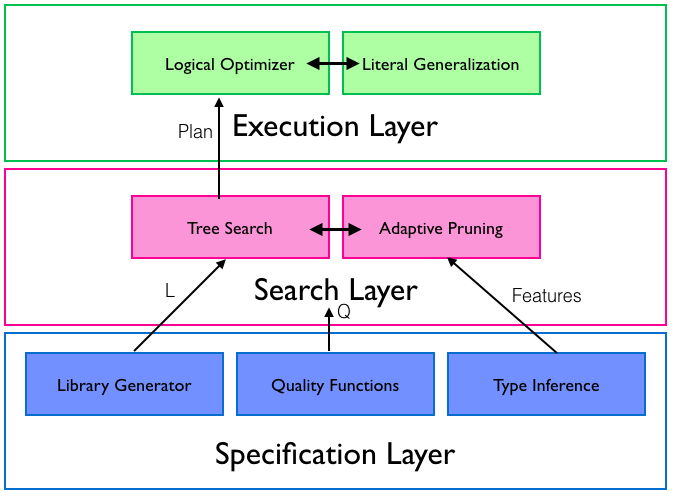
\includegraphics[width=\columnwidth]{figures/alphacleanarch.png}
 \caption{ \sys is given a specification of quality (e.g., integrity constraints or a statistical model the data must conform to) and a language  of  allowed  data  transformations,  and  it  searches  to find a sequence of transformations that maximizes the quality metric. \label{fig:arch} }
\end{figure}


\Cref{fig:arch} depicts the \sys system architecture, consisting of three main components.  The {\it Interface} takes as input domain-specific cleanliness measures and data cleaning operations that the user provides  and translates them into a quality function and data transformation language.   For instance, our current implementation supports a wide range of quality functions including: attribute type constraints, functional dependencies, denial constraints, lookup tables~\cite{}, parametric and non-parametric outlier models, and correlations between numeric attributes.  Our existing cleaning data transformations primarily focus on conditional cell and record transformations that apply a transformation to all cells or records that satisfy a predicate; both the transformation parameters and the predicate are learned by \sys.  \Cref{s:appendix} provides a detailed description of the supported functions and extendible API. 

The {\it Search} component takes as input $Q$ and $L$, and performs a greedy search heuristic to find a program $p^* \in L$ that maximizes $Q$.  Users can supply hints that exploit the problem structure to reduce the runtime by pruning the search space and parallelizing the search.  \sys supports two main classes of pruning-based optimizations. {\it Static} rules that invalidate programs in $L$ that are unlikely to be useful.  For instance, composing the same idempotent transformation (e.g., \texttt{find\_replace(SFO, SF, city\_name)}) is redundant and can be immediately skipped.  {\it Dynamic} rules have access to the result of a candidate program when making pruning decisions, and we propose a novel approach to learn automatic dynamic pruning rules that can reduce end-to-end runtimes by up to \ewu{XXX} at the expense of slightly lower recall.  \Cref{s:search} describes the pruning rules and parallelization optimization in detail.


Finally, once search component outputs the cleaning program $p^*$, the {\it Program Optimizer} optimizes $P^*$ provides an API to apply simple query compilation techniques.  \sys currently replaces variables with literal values whenever possible.  In addition, we implement loop fusion~\cite{} to avoid scanning the input and intermediate relations for each transformation in $p^*$. Finally, we inline the data transformation functions into the loops.    

For example, consider the operations from~\Cref{ex3}.  Since the \texttt{find\_replace} operations do not conflict, it is inefficient to loop through over the relation instance three separate times.  
Since they do not conflict, it would be inefficient to execute them sequentially and iterate over the data three separate times.
Instead, one should combine the operations together and execute at once:
\begin{lstlisting}
for r in rows:
 if r[city_name] == `New York':
   r[city_name] = `New York City'
 elif r[city_name] == `San Francisc':
   r[city_name] = `San Francisco'
 if r[city_code] == `NYC'
   r[city_code] = `NY'
\end{lstlisting}
We find that even these simple optimizations improve the final program runtime by \ewu{XXX}, and leave further improvements to future work.


% The user can optionally provide custom quality functions and data transformations as simple Python class definitions.      takes as input user specifications of the quality function and data transformation language, alongside search configuration parameters.


\if{0}
Now, we will overview some of the preliminary concepts and describe how this formalism inspires a modular system API.
\sys is designed as a software stack with three layers: a specification layer, a search layer, and an execution layer.
To understand how these layers interact, we will use the example in Section 2 throughout this section.


\subsection{Specification Layer} The provides an API for specifying a quality function and a language of transformations. This allows one to specify a data cleaning problem for a particular dirty instance. As described in the previous section, we provide an API for translating common data cleaning specifications, constraints, statistical models, and gold standard examples, into quality functions. 

The harder problem is specifying the language. 
The challenge is that most data transformations are parametrized by literal values from the database.
We need efficient techniques to automatically enumerate this transformation set before we apply the search.
The language is generated through a transformation templates which are dynamically populated by literals in the database.
A template is a parametrized transformation:
\[T(R, [\theta_1, \theta_2,...,\theta_k] ): \mathcal{R} \mapsto  \mathcal{R},\] where the parameters $[\theta_i]$ are populated by literal values.
Each $\theta_i$ represents an SQL query except for special parameters such as attribute names and data-independent hyperparameters.
The system dynamically generates all possible literal instances of this transformation by taking the cartesian product of the query results.

In the running example, consider the following function:
\[
\textsf{find\_replace}(\text{source}, \text{target}, \text{attribute})
\]
\begin{lstlisting}
source := SELECT attribute from R;
target := SELECT attribute from R;
\end{lstlisting}
Likewise for numerical transformations, consider the function that clips outlier values outside 6 standard deviations of the mean:
\[
\textsf{clip}(\text{mean}, \text{threshold})
\]
\begin{lstlisting}
mean := SELECT mean(attribute) from R;
threshold := SELECT 6*std(attribute) from R;
\end{lstlisting}
\sys provides queries and filters for a number of common parametrizations or they can be specified manually.

\subsection{Search Layer (Section 5)} The next layer is the search layer, which implements the basic search algorithm of \sys. This algorithm is a distributed best-first greedy search.  
With no additional information, the search approach described would have to evaluate $61^3 = 226981$ transformations, which is clearly impractical even for this small example.
This layer also provides an interface for custom search optimizations:

\vspace{0.5em}\noindent\textbf{Static Optimizations: } A static optimization is a regular expression that all transformation sequences must satisfy independent of the data. 
\[\textsf{static\_opt}(L, \text{regex} ) \mapsto L'\]
For example, since the find-and-replace operations are idempotent, i.e., $T(T(R)) = T(R)$, we may want to only consider the set of all sequences with no neighboring repeated transformations. Similarly, we may also want to prune all search branches that make no effect (i.e., find-and-replace New York with New York).
These two regular expressions alone reduce the overall number of evaluations by $48\%$ in the above example (120050 v.s. 226981 evaluations).
There are several other possible optimizations  such as avoiding changes that reverse previous changes $T_i(T_j(R)) = R$.


\vspace{0.5em}\noindent\textbf{Dynamic Optimizations: } A dynamic optimization can query the data and cost function to generate rules that are instance-specific:
\[\textsf{dyn\_opt}(Q, R, L) \mapsto \text{regex}\]
For example, we may want to ensure that all the evaluations are ``correlated'' with the cost function--that is it makes modifications that are likely to affect the costs.
This is possible if the cost separable where we have a score for each cell. In this case, we can find all the cells in violation of the functional dependencies and make sure that the ``source'' field of the find-and-replace operations only match values that are in violation.
These optimizations are called ``dynamic' because they can be determined from the active domain (i.e., after applying a transformation, recalculate new optimization rules).
Applying this optimization (in addition to the others) to the example reduces the search space to 1582 evaluations v.s. 226981 unoptimized (143x reduction).

\vspace{0.5em}\noindent\textbf{Blocking Rules: }  Arbitrary constraint satisfaction problems are challenging because all variables can interact. While this is certainly the case for arbitrary quality functions, in many cases, data errors are localized. For example, replacing \texttt{San Francisc} with \texttt{San Francisco} has no effect on the records referring to \texttt{New York City}. The final class of optimizations are blocking rules which have been widely used in entity resolution systems:
\[\textsf{block}(Q, R, L) \mapsto \{R_1,...,R_k\} \]
For quality functions generated from dependencies, we can determine blocks analytically--looking at which violating tuples are linked through the constraint.
However, in general, these blocking rules can be learned (e.g., with clustering) or user defined.
The search can execute on each of the blocks independently.
\fi

\section{Search Overview}
This section describes \sys's search algorithm and optimizations in greater detail.    

% The optimization algorithm takes a quality function, a language, and a dirty relation, and outputs a sequence of transformations (of max depth $k$) that maximizes the quality function.

\begin{algorithm}[t]
\KwData{Q, R, L, (k, $\gamma$)}

// Initialize priority queue of candidate programs\\
$O = \{NOOP\}$

\While{ $\exists ~ o \in O: \|o\| < k$ }
{
    \For{$o \in O: \|o\| < k$ }{
        
        Pop $o$ from the queue.
        
        \For{$t \in L$}{
             $o' = o \circ t$ 
             
             Push $o'$ with priority $\bar{Q}(o'(R))$.
        }
    }
    
    Pop all elements from with a priority greater than $\gamma$ times the lowest value in the queue.
}

\Return Lowest item on the queue
\caption{Greedy Best-First Tree Search \ewu{turn O and o into P and p to be consistent with background}}
\label{alg:main}
\end{algorithm}

\subsection{Naive Search Procedures}
In principle, any tree search algorithm over $L$ would be correct.
However, the traversal order and expansion policy is important in this search problem.  We describe the algorithmic and practical reasons why two naive procedures---breadth-first search (BFS) and depth-first search (DFS)---exhibit poor search runtimes.

\stitle{BFS} This approach extends each program in the search frontier with every possible data transformation in $\Sigma$.  To extend a candidate program $l_c$ with $T \in \Sigma$, it evaluates $Q((T\circ l_c)(R))$.  Unfortunately, the frontier grows exponentially with each iteration.  Additionally, evaluating every new candidate program $T\circ l_c$ can be expensive if the input relation is large.   Although the cost can be reduced by materializing $l_c(R)$, it is not possible to materialize all candidate programs in the frontier for all but the most trivial cleaning problems.    It is desirable to use asearch procedure that bounds the size of the frontier and the materialization costs.

% The first problem with this algorithm is that since each node in this tree $o$ represents a sequence of transformations.
% Evaluating the value of $o$ can be very expensive since it would have to evaluate the entire path to the root.
% $o$ is a composition of many transformations and may require a number of passes over the dataset.
% This can be avoided if we can materialize (either to disk or memory) the frontier,that is, for each node in the priority queue $o \in O$, we have a cached result of $o(R)$. 
% However, with BFS, the frontier is expoential in the support of the language and the system would quickly run out of memory.

\stitle{DFS} Depth-first search only needs to materialize the intermediate results for a single program at a time, however it is highly inefficient since the vast majority of programs that it explores will have low quality scores.  

\subsection{Basic Algorithm}
A best-first search expands the most promising nodes chosen according to a specified cost function.
We consider a greedy version of this algorithm, which removes nodes on the frontier that are more than $\gamma$ times worse than the current best solution.
Making $\gamma$ larger makes the algorithm asympotically consistent, whereas $\gamma=1$ is a pure greedy search.

The algorithm is described in Algorithm \ref{alg:main}.
The algorithm is initialized with an identity transformation. This identity transformation is placed on a priority queue where the priority is the aggregate quality after applying the transformation (in this case the quality of the original relation $R$).
Then, the algorithm ``expands'' all elements on the queue with description length of less than $k$.
By expansion, we mean that it removes the element from the queue composes the element with a transformation from the library.
Then, it places the new composed transformation onto the priority queue with its new quality score as the priority.
The algorithm then flushes the priority queue of all elements with priority more than $\gamma$ times worse than the current best solution.
This process repeats until all elements on the queue have a description length of $k$.

We can materialize (either to disk or memory) the frontier,that is, for each node in the priority queue $o \in O$, we have a cached result of $o(R)$. 
Then, when we expand the nodes to $o' = o \circ t$, we only have to incrementally evaluate $t(R)$.
After the node is expanded, the result is added to the cache if it within $\gamma$ of the best solution.
The basic algorithm described above is well-suited for this problem.
Without the greediness, the frontier might be exponentially large leading to an impractical amount of materialization.
By tuning $\gamma$, the user can essentially set how much memory is used for materialization.

\begin{figure*}
    \centering
    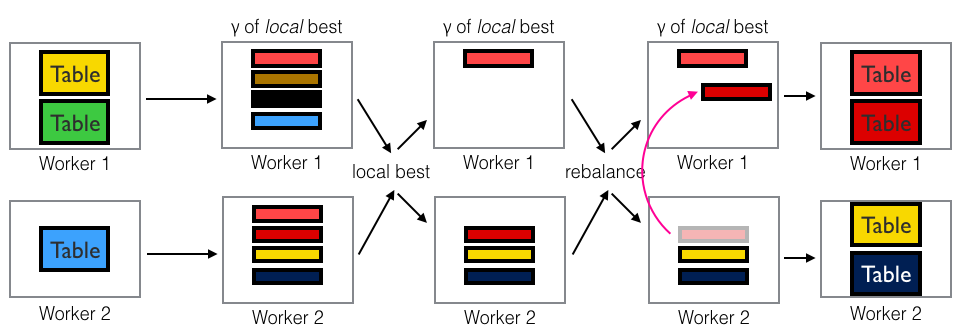
\includegraphics[width=0.6\textwidth]{figures/distributed.png}
    \caption{TODO}
    \label{fig:my_label}
\end{figure*}

\subsection{Optimizations Overview}

\stitle{Static Pruning} A static optimization is a regular expression that all transformation sequences must satisfy independent of the data. 
\[\textsf{static\_opt}(L, \text{regex} ) \mapsto L'\]
For example, since the find-and-replace operations are idempotent, i.e., $T(T(R)) = T(R)$, we may want to only consider the set of all sequences with no neighboring repeated transformations. Similarly, we may also want to prune all search branches that make no effect (i.e., find-and-replace New York with New York).
These two regular expressions alone reduce the overall number of evaluations by $48\%$ in the above example (120050 v.s. 226981 evaluations).
There are several other possible optimizations  such as avoiding changes that reverse previous changes $T_i(T_j(R)) = R$.


\stitle{Dynamic Pruning} A dynamic optimization can query the data and cost function to generate rules that are instance-specific:
\[\textsf{dyn\_opt}(Q, R, L) \mapsto \text{regex}\]
For example, we may want to ensure that all the evaluations are ``correlated'' with the cost function--that is it makes modifications that are likely to affect the costs.
This is possible if the cost separable where we have a score for each cell. In this case, we can find all the cells in violation of the functional dependencies and make sure that the ``source'' field of the find-and-replace operations only match values that are in violation.
These optimizations are called ``dynamic' because they can be determined from the active domain (i.e., after applying a transformation, recalculate new optimization rules).
Applying this optimization (in addition to the others) to the example reduces the search space to 1582 evaluations v.s. 226981 unoptimized (143x reduction).

\stitle{Parallelization}  Arbitrary constraint satisfaction problems are challenging because all variables can interact. While this is certainly the case for arbitrary quality functions, in many cases, data errors are localized. For example, replacing \texttt{San Francisc} with \texttt{San Francisco} has no effect on the records referring to \texttt{New York City}. The final class of optimizations are blocking rules which have been widely used in entity resolution systems:
\[\textsf{block}(Q, R, L) \mapsto \{R_1,...,R_k\} \]
For quality functions generated from dependencies, we can determine blocks analytically--looking at which violating tuples are linked through the constraint.
However, in general, these blocking rules can be learned (e.g., with clustering) or user defined.
The search can execute on each of the blocks independently.
\ewu{Emphasize that this is based on the decomposable nature of the quality function}

\stitle{Quality Estimation}  A large cost to the search algorithm stems from the need to execute the quality function over the output of each candidate program.  In some cases, it is possible to estimate the quality function without fully running the candidate program.  For instance, \ewu{foofah}.  Alternatively, it may be sufficient to run the candidate program over a sample of the input relation.  These are opportunities for future work.

\section{Search Optimizations}
\subsection{Parallelism}
The best-first search algorithm also is amenable to parallelization. One can parallelize over the two inner for loops $O \times L$. Each expansion can be forked into its own thread. However, this actually makes the materialization described above a bit more challenging. 

\subsubsection{Shared Memory Parallelization}
The most straight-forward case is when we have access to low-latency shared memory between the expansion threads. In each expansion round, the main thread will assign each expansion node to workers and they will evaluate a given transformation. Each worker will make a copy of $o(R)$ (the node it is expanding) into shared memory. 
If the expanded transformation is within $\gamma$ of the best current result, then it will update the copy, otherwise delete it. The point of synchronization is after all expansions are finished, and the main driver will flush all transformations less than $\gamma$ of the best result, and then assign new workers for the next round. 

\subsubsection{Distributed Parallelization}
In cases, where we do not have access to low-latency shared memory, the communication costs of the above algorithm can be impractical. For each expanded node, the entire table has to be communicated to each of the distributed nodes.
We consider a worker-driver model, and assume that the number of workers is $k$.

\vspace{0.25em} \noindent  \textbf{Initialization. } 
Each worker has a copy of the base relation with no transformations.
In the first round of expansion, the driver assigns to each worker $\frac{|L|}{k}$ expansions. 
Each worker executes each of its assigned expansions, and stores the transformations that are within $\gamma$ of the best local result.

\vspace{0.25em} \noindent  \textbf{Reconciliation. }  Note that the global top-$\gamma$ set is a subset of the union of the all local results.
The workers then communicate the quality of their best transformation. This can be used to reconcile the local materializations to only the global top-$\gamma$ set.
This set is not necessarily balanced, e.g., one worker might have almost all of the top transformations.
The next step is a balancing step, where each worker communicates the number of materialized expansions it currently stores.
The workers with more than $\frac{|O|}{k}$ materialized expansions  randomly select ones to evict, and the driver re-distributes these to nodes with too few materialized expansions.
This is done by communicated the transformation and the result is re-computed on the new worker.
If $|O| < k$, then expansions are chosen at random to be replicated.
The result of the reconciliation step is that all workers have an evenly distributed set of materialized expansions.

\vspace{0.25em} \noindent  \textbf{Next Round. } After reconciliation, each worker is associated with a particular $o \in O$ (or a set of them). To parallelize, the driver must simply ensure that it assigns new expansions only to those workers that have materialized the parent.
The algorithm then repeats, expanding each node locally, and then reconciles the results.









\subsection{Learning Dynamic Pruning Rules}
To effectively search through the language of transformations, search heuristics are important.
However, it can be challenge to devise these heuristics \emph{a priori}.
This section describes how Machine Learning can be used to learn a search heuristic as data is cleaned.

\subsubsection{Motivation}
The search algorithms in  most automatic data cleaning frameworks are carefully tuned for a specific quality function or class of quality functions. For example, the chase used in functional dependency resolution does not make an edit to the table unless it enforces at least one tuple's FD relationship. Exploiting the structure of the specific problems allows for a tractable solution technique. Similarly, in entity matching problems, one restricts the search to only matching tuples that are likely to be similar based on some similarity metric.
These are not static optimizations, i.e., knowing how to prune the search space requires knowing the underlying data or making strong modeling assumptions about the types of transformations used.

\subsection{Algorithm \ewu{(Give a name?)}}
\sys executes the search on each block of data.
The result is a sequence of transformations to optimize the quality metric on that block.
Every transformation in this sequence can be treated as a positive training example $L^+$, and every transformation not in this sequence can be treated as a negative example $L^-$.
The idea is that if we apply the search to a sufficient number of blocks then we can train a classifier to predict whether a transformation will be included in the final sequence.
It is important to note that this prediction is over the transformations and not the data. 

Internally, \sys uses a Logistic Regression classifier to make this classification. The Logistic Regression is tuned towards False Positives (i.e., keep a bad search branch). This is done by training the model and shifting the prediction threshold until there are no False Negatives. 


\subsection{Non-numerical Attribute Support}
Suppose we made only the following assumption about the language of transformations used.
Each transformation consists is described by a fixed-length feature vector in $\mathbb{R}^k$:
\[
\textsf{feat}: T \mapsto \mathbb{R}^k 
\]
An example of a featurization, consider a transformation from the the running example:
\begin{lstlisting}
find_replace(New York, New York City, city_name)
\end{lstlisting}
The featurization could encode the string similarity of the two literal parameters and an indicator vector describing which column it applies to.

Consider an alternative to a predefined search heuristic where we clean data in small blocks.
For the initial blocks, we search without a heuristic.
As we continuously perform the search, we train a classifier on these features to reject search branches that are not typically in the final solution.
This allows us to exploit any patterns in the literal parameters that repeatedly occur.

For example, some columns might not be dirty and are not worthwile to clean.
In the example above, another observation could be that the source and target strings in the optimal sequence are very close in terms of string similarity (as opposed to arbitrary transformations).
If each of these operations was featurized with a single scalar that is the edit-distance between the two strings, then the classifier could learn a pruning threshold (i.e., not considering find-and-replace operations above that threshold).



\section{Experiments}\label{s:exp}
In this section, we present the results of our experiments.  We execute \sys on $12$ datasets based on three sets of real-world cases---machine learning competitions, data analysis pipelines, and \company---and report accuracy measures and end-to-end runtime.  Then, we present a series of micro-benchmarks that evaluate each of the modules of \sys.  Our goal is to understand the conditions where automated cleaning is able to accurately detect and repair data in a way that improves the held-out test accuracy. 

In particular, we evaluate three hypotheses: 1) Compared to baselines, the cleaning operations selected by \sys result in a greater improvement to the downstream classification accuracy; 2) \sys automatically detects a large fraction (in comparison to hand-written rules) of the errors across several different datasets; and 3) The optimizations that we design for \sys allow us to run at a reasonable wall clock time.

\subsubsection{Setup}

To the best of our knowledge, there does not exist a comparable general purpose ML+Data Cleaning system to \sys in industry or academia.  We evaluate \sys against a number of baseline approaches inspired by solutions proposed in literature.   These baselines are described in the subsequent experimental subsections.
We used the following setup for our experiments. 

\stitle{Test Data: } For each of the datasets, we defined a 20\% held-out test dataset. We assumed that the labels in this test dataset were clean, as per the assumption in \sys. To avoid overfitting, we carefully designed the accuracy evaluation experiments for \sys by using a ``doubly'' held out test dataset: the test dataset used to optimize \sys is different from a completely unseen 20\% test dataset that is solely used to report the final prediction accuracy.
Training is performed on the remaining 60\% of the data.

\stitle{Models: } We used the \textsf{sklearn} Random Forest classifier.  The training procedure uses a set of standard featurizers (hot-one encoding for categorical data, bag-of-words for string data, numerical data as is) in a similar fashion as~\cite{gokhale2014corleone}.  Note that these featurizers are used as part of the black-box training procedure and are distinct from those used in the detector generator library. 
We describe hyper-parameter settings for each technique in the text of each experiment.
As much as possible, we attempted to use the library default parameters.

\stitle{Timing: } In all of our experiments, we used standard classification models and featurization techniques from Python \textsf{sklearn}.
The classifiers were trained in Python 2.7 and timing experiments were run on an Amazon EC2 m4.16xlarge instance\footnote{64 virtual cpus and 256 GiB memory}.







\begin{table*}[t]
\centering
\begin{tabular}{|l|r|r|r|r|r|r|r|r|r|r|r|}
\hline
ML Competition& \#rows & \#cols & NC & Q &	IC & Q+IC &	Best-1 &	Worst-1 &	BC-3 & BC5 & Abs. Improvement\\
\hline
USCensus	&32561&15&0.85&	0.82&	0.86&	0.84&	0.87&	0.79&	0.88&	\pop{0.91} & +0.04\\
Emergency &11176&9&	0.67&	0.72&	0.67&	0.72&	0.72&	0.66&	0.72&	\pop{0.75} & +0.03\\
Sensor	&928991&5&0.92&	0.93&	0.92&	0.89&	0.92&	0.8&	\pop{0.94}&	0.94 & +0.01\\
NFL	&46129&65&0.74&	0.74&	0.76&	0.75&	0.76&	0.74&	0.79&	\pop{0.82}& +0.06\\
EEG	&2406&32&0.79&	0.82&	0.79&	0.83&	0.83&	0.7&	0.85&	\pop{0.89}& +0.06\\
Titanic	&891&12&0.83&	0.72&	0.83&	0.76&	0.83&	0.69&	0.83&	\pop{0.84}& +0.01\\
Housing	&1460&81&0.73&	0.76&	0.73&	0.77&	0.77&	0.65&	\pop{0.81}&	0.76& +0.04 \\
Retail	&541909&8&0.88&	0.88&	0.91&	0.91&	0.91&	0.87&	0.94&	\pop{0.95}& +0.04 \\
\hline
\hline
Data Analytics &\#rows & \#cols & NC & Q &	IC & Q+IC &	Best &	Worst &	BC-3 & BC5 & Abs. Improvement\\
\hline
FEC  & 6410678 & 18 & 0.62 & 0.53 & 0.61 & 0.57 & 0.71 & 0.51 & 0.74 & \pop{0.77} &  +0.06 \\
Restaurant (Multiclass) &758&4& 0.42 & 0.42 & 0.58 & 0.68 & \pop{0.62} & 0.36 & 0.61 & 0.60 & (-0.02) \\
\hline
\hline
Company X &\#rows & \#cols & NC & Q &	IC & Q+IC &	Best &	Worst &	BC-3 & BC5 & Abs. Improvement\\
\hline
Dataset 1 (AUC) &76684&6&0.60&0.60&0.60&0.60&0.61&0.59&0.66&\pop{0.69}& +0.08 \\
Dataset 2 (AUC) &83986&6&0.55&0.55&0.52&0.55&0.55&0.52&0.61&\pop{0.63}& +0.09\\
\hline
\end{tabular}
\caption{End-to-end accuracy results for each dataset and experimental method. We report standard classification accuracy.  The right column summarizes the absolute accuracy improvement over the best non BC-3/5 approach.  The \company datasets have high class imbalances cause artificially high accuracy statistics,  so we report AUC statistics for those datasets instead.}
\label{tab:accuracy}
\end{table*}

\subsection{End-to-End Accuracy}
In our first experiment, we evaluated the accuracy of \sys compared to the baselines.
We tried to minimize hyper-parameter tuning as much as possible to simulate a real-scenario where extensive tuning and parameter search might be expensive.

\subsubsection{Methods}

\stitle{No Cleaning (NC): } We train a model without any modification to the training or test data.

\stitle{Quantitative (Q): } We train a model where only the isolation forest over the numerical attributes is used to detect errors.
Errors in both training and test are imputed with a mean value.

\stitle{Integrity Constraint (IC): } We read through each dataset to identify a set of anomalous values for each non-numerical attribute on a best-effort basis.  We then codified these as integrity constraint rules, and corrected the identified errors using a statistical distortion minimization metric as in~\cite{prokoshyna2015combining}. Statistical distortion minimizes the statistical distance to some ideal distribution (e.g., Power Law or Gaussian). We set these distributions manually by inspecting the data when possible.

\stitle{Quantitative + IC (Q+IC): } We use both the quantitative and integrity constraints for detection. For repair, we apply an imputation with a default value. For categorical and string-valued attributes, this the most frequent value. For numerical attributes, this is the mean value.

\stitle{Best Single (Best-1): } We run \sys with $B=1$ and identify the  single best conditional repair.

\stitle{Worst Single (Worst-1): } We run \sys with $B=1$ and identify the single worst conditional repair..

\stitle{BC-3: } We run \sys with $B=3$.

\stitle{BC-5: } We run \sys with $B=5$.

\subsubsection{ML Competition Datasets}\label{exp:comp}
We downloaded 8 binary classification datasets from Kaggle competitions and benchmarks in the UCI ML repository.  
These datasets have been extracted, structured, and published.
Nevertheless, they contain missing values, numerical outliers, and pattern errors (oddly formatted values).
For this set of experiments, we used a single hyper-parameter setting for all the detectors and classification models (default \textsf{sklearn} library setting). 
%\ewu{IMPORTANT: SOMEWHERE IN THE WRITING, WE FORGOT TO TALK ABOUT HYPERPARAMETERS}
We briefly describe each dataset and their errors below:

\vspace{0.5em}\noindent\textbf{USCensus: } This dataset contains US Census records for adults and the goal is to predict  whether the adult earns more than $50,000$ dollars. It contains 32,561 records with 15 numerical and categorical attributes. This dataset contained missing values and coding inconsistencies.

\vspace{0.5em}\noindent\textbf{NFL: } This dataset contains play-by-play logs from US Football games. The dataset contains 46,129 records with 65 numerical, categorical, and string-valued attributes. Given the record, the classification objective is to determine whether the next play the team runs is a run or a pass play.
The dataset contains a significant number of missing values and ``sentinel'' records that mark the end of a log sequence. The sentinel records do not signify a play but rather signify a timeout, end of quarter, or end of the game.

\vspace{0.5em}\noindent\textbf{EEG: } This is a dataset of EEG recordings. 
The training data is organized into ten minute EEG clips labeled "Preictal" for pre-seizure data segments, or "Interictal" for non-seizure data segments. 
There are 2406 records each of which is a variable-length time-series of 16 attributes. We featurize this dataset into records of 32 attributes--the mean and variance over the length of the time-series. 
This dataset primarily contains numerical outliers, the clips have spurious readings.

\vspace{0.5em}\noindent\textbf{Emergency: } This dataset contains records on 911 calls from Pennsylvania. There are 111,766 records with 9 attributes. Given the record, the classification challenge is to determine whether the emergency service response time will be less than $5 min$. This dataset contains missing values, and spurious locations not served by the 911 center.

\vspace{0.5em}\noindent\textbf{Sensor: } The Intel sensor dataset~\cite{data, DBLP:journals/pvldb/0002M13, wang1999sample} contains 928,991 temperature, humidity, and light sensor readings a sensor deployment. The classification task is to predict whether the readings came from a particular sensor (sensor 49). This dataset primarily has numerical outliers.

\vspace{0.5em}\noindent\textbf{Titanic: } This dataset contains 891 records from the Titanic manifest with 12 attributes. The classification objective is to determine whether the passenger survived or not. There are missing values and string formatting errors.


\vspace{0.5em}\noindent\textbf{Housing: } The housing dataset contains 1460 records and 81 attributes of house price listings. The classification objective is to determine whether the listed house will be sold above 750000. 
This dataset contains missing values as well as numerical outliers.

\vspace{0.5em}\noindent\textbf{Retail: } The online retail dataset contains 541,909 records of online retail purchases with 8 attributes. The classification objective is to predict whether the purchase occurred in the United Kingdom.
This dataset contains numerical errors where some purchased quantities are reported as negative.


\vspace{1em}
The first set of rows in Table \ref{tab:accuracy} present the predictive accuracy of models trained with \sys on the completely unseen test data.  In all experiments, the model trained with one of the \sys  approaches was the most accurate.
The quantitative baseline performed well when the errors were clear numerical outliers (e.g., Sensor and  EEG).  However, its performance suffered in datasets with missing values or formatting errors, and {\it degraded model accuracy} in the US Census dataset.
Conversely, the integrity constraint approach worked well for non-numerical errors, however it was not useful for Emergency, EEG, Housing, nor Sensor.
The naive union of (Q+IC) has difficulty composing the two operations in the US Census dataset and degrades accuracy as compared to quantitative or integrity constraint alone in several datasets.  Finally we compare and find up to a 14\% difference between the best and worst repairs when using \sys.  These results emphasize the need for an automatic search solution that can avoid repairs that are ineffective or reduce accuracy.

BC-3 and BC-5 improve the predictive performance of the models.
In all of the datasets, we found that either BC-3 or BC-5 had the highest test accuracy.
There is an interesting reason why BC-3 is more accurate than BC-5 in two cases.
Consider the case where there are only three types of errors in the dataset.
Then BC-3 would in principle select cleaners to address them. The remaining two cleaners would just add noise.
Our evidence suggests that this happened in the two datasets where the errors were mostly concentrated on a handful of attributes.

\subsubsection{Data Analytics}
The next class of datasets that we considered were datasets known to have significant errors--unlike the relatively clean competition datasets. These are two datasets that were used in previous data cleaning papers, and we designed classification tasks based on the datasets.
Unlike the ML competition datasets, we tuned the classifier and detector hyperparamters for each dataset. 
The accuracy results are presented in the second set of rows in Table \ref{tab:accuracy}.

\vspace{0.5em}\noindent\textbf{Federal Election Commission Contributions: } The FEC provides a dataset of election contributions of 6,410,678 records with 18 numerical, categorical and string valued attributes. This dataset has a number of errors. There are missing values, formatting issues (where records have the wrong number of fields causing misaligment in parsing), and numerical outliers (negative contributions).

Our classification objective was to determine whether the contribution would be above or below $100$ dollars. Due to the severity of the errors in the dataset, there is nearly a 15\% difference between the prediction accuracy of a classifier with and without \sys.
Furthermore, a purely quantitative approach is not useful for this dataset.
An integrity constraint based method improves accuracy but the automatic imputations are unreliable on this data.
Furthermore, it is difficult to express a problem like row misalignment as a integrity constraint.

We find empirically that the alignment is better detected by the word2vec error detector in \sys.
As a result the best single cleaner is using the word2vec error detector.
This is improved by combining this with quantitative checks for numerical outliers and missing values.
In all, \sys with a budget of 5 improves accuracy 8.4\% over the best single cleaner. 

\vspace{0.5em}\noindent\textbf{Restaurant Dataset: } The restaurant dataset has 758 distinct records and 4 attributes. This dataset has typically been used as a benchmark for entity resolution since records are duplicated with minor inconsistencies.
We designed a multi-class classification task to see if we could predict the city from record.
One of the major inconsistencies was additional attributes appended to the restaurant category.

On this dataset, we see a negative result from \sys. Our test error decreases as we increase the number of selected cleaners. We speculate this is due to overfitting due to the extremely small size of the dataset  ($<1000 records$) combined with the expressiveness of the classifiers model.

\subsubsection{Company X Experiments}
A researcher at \company ran \sys on two production datasets using the same model and the same parameters (random forest classifier) that are deployed in the company.  The datasets contain 76,684 and 83,986 records respectively, and both contain six attributes that are inferred as categorical attributes.  These datasets are interesting due to a significant class imbalance, where most records were labeled $0$ (no sale) and very few were labeled $1$ (successful sale).
Because of this imbalance, the accuracy of simply predicting $0$ performs nearly perfectly, and we instead report the AUC classification score.  Furthermore, due to data confidentially, we were only able to acquire aggregate statistics about the data cleaning results.  The detailed AUC results are reported in the last set of rows in  Table \ref{tab:accuracy}.

In these two datasets, the primary errors were detected by the missing values and word2vec featurizers. 
\sys detected 50\% (40,164) and $95\%$ (80,168) of the rows in their respective datasets as containing missing values, anomalous categorical values, or both.  
\sys with 5 selected cleaners achieves an absolute improvement of $8-9\%$  in both datasets over the next best non-\sys alternative, and a slightly larger improvement over not cleaning the dataset at all.
% It achieves a 9\% absolute improvement over no cleaning in dataset 1 and a 8\% improvement in dataset 2.
Interestingly, we found that the integrity constraint approach (IC) reduced the AUC results in dataset 2, however due to confidentiality, we do not know the reason at the time of submission.


\begin{figure}[t]
\centering
\includegraphics[width=0.8\columnwidth]{exp/runtime.png}
\caption{Training runtime on a 6M record dataset (1.5GB). The repair selection scales due to the parallelization optimization, however we did not parallelize the other steps.\label{exp:runtime}}
\end{figure}

\begin{figure}[t]
\centering
\includegraphics[width=0.8\columnwidth]{exp/runtime2.png}
\caption{Prediction throughput is significantly higher than training throughput (Figure~\ref{exp:runtime}).  Reported for 16-cores.\label{exp:tp}}
\end{figure}

\subsection{End-to-End Run Time}
Next, we evaluate the end-to-end wall clock runtime of \sys. We use the FEC dataset since it is the largest. This evaluation includes all of the optimizations for \sys. The FEC dataset is 1.5 GB (about 6M records). 
Figure \ref{exp:runtime} plots the results.
With a single core, \sys takes 2422 seconds in wall-clock time. Of that time, 2072 seconds is spent in repair selection, 306 seconds is spent in error detection, and 44 seconds in loading the dataset.
We can parallelize the repair selection step. We parallelize the inner-loop of the boosting algorithm. On 16-cores, we are able to reduce the runtime of the repair selection to 212 seconds. This constitutes a 9.7x speedup for that step.

It is important to note that this latency is only incurred during training. During prediction, the learned model can be applied, and this process is much faster than training. 
Figure \ref{exp:tp} plots the throughput of \sys.
The number of records that can be processed per second on 16 cores for prediction is 19746 records/second, but during training it is 9316 records/second. One of the key bottlenecks is evaluating the word2vec model for each prediction, and without this model, the throughput increases to 23746 records/second.

\begin{figure}[t]
\centering
 \includegraphics[width=\columnwidth]{exp/daccuracy.png}
 \caption{ \sys achieves up to 81\% accuracy and is competitive with hand-written rules, and the word embedding features significantly improve the detector accuracy.
 \label{fig:derror}}
\end{figure}

\begin{figure}[t]
\centering
 \includegraphics[width=\columnwidth]{exp/druntime.png}
 \caption{Runtimes for 8 Machine Learning competition datasets as in Figure~\ref{fig:derror}. \sys is slightly slower than hand-written rules, and much faster than MCD.
 \label{fig:druntime}}
\end{figure}

\subsection{Detector Micro-Benchmarks}

We used a set of error detectors based on heuristics, statistical methods, the word2vec neural network, and evaluated their accuracy and runtime as compared to hand crafted rules (Custom).  We evaluated typical outlier detection techniques such as Minimum Covariance Determinants (MCD) and Isolation Forests with naive hot-one encoding for categorical attributes (ISO).  We also evaluated \sys by incrementally the set of featurizers that are used: quantitative only (BC-Q), with  missing value featurizers (BC-Q,MV), with word embeddings (BC-all).  We report the F1 score on the 8 machine learning datasets.

Figure  \ref{fig:derror} shows that the final detector in \sys achieves up to 81\% of the accuracy of hand-written rules on the competition datasets.
Confirming the results of Abedjan et al.~\cite{DBLP:journals/pvldb/AbedjanCDFIOPST16}, we found that a 
purely quantitative approach does not perform well in comparison to the rule-based approach on these datasets (Isolation Forest alone and MCD).
However, results are significantly improved when combined with heuristics that detect missing values. 
The performance gap is even further reduced when the detector additionally uses a Neural Network to learn how attributes correlate with each other, and detect anomolous correlations.
It is important to emphasize that these datasets represent a very specific domain, i.e., structured training datasets for ML.
The datasets are already in a structured schema and the only thing that an analyst has to worry about is handling inconsistent attribute values.
Presumably these datasets were also previously cleaned and extracted before they were publicly released.
Our initial experiment showed that for this class of datasets, reasonably accurate error detection is possible with minimal supervision and tuning.

 Figure  \ref{fig:druntime} shows the total runtime (training and test) of each  approach.
 We first apply the Minimum Covariance Determinant approach (MCD) to the set of records featurized ``naively''--numerical values, hot-one encoded categorical values, and bag-of-words for strings.
 We found that MCD was very expensive since this featurization increases the dimensionality significantly and MCD needs to compute an $d^2$ covariance matrix.
 Next, we apply the Isolation Forest to the same featurization.
 The Isolation forest is up-to $50x$ faster than MCD on the same features.
 This was one of the big motivations for using an isolation forest internally in \sys.
 
 After that, we applied Isolation Forests to progressively more of the featurizers used by \sys.
 First, we applied it just to the numerical attributes--this is the fastest.
 Then, we applied it to numerical attributes, missing values, and parsing errors--this adds $1.5x$ overhead on averaage.
 Finally, we added in the word2vec neural network features (excluding training time for the Neural Network).
 We notice that with this featurization the Isolation Forest is faster than the one with the naive featurization due to the lower dimensionality.
 Of course, rules are faster to evaluate than a learning detector and this gap was on average a factor of 3.
 
 \begin{figure}[t]
\centering
 \includegraphics[width=0.9\columnwidth]{exp/opt1.png}
 \caption{This plot (log scale) shows the impact of optimizations on the selector's runtime. Materialization and Indexing allow the algorithm to scale with the number of selected cleaners. Otherwise, the algorithm repeatedly retrains and recleans the same data.
 \label{fig:opt}}
\end{figure}
 
 \subsection{Repair Micro-Benchmarks }
 
 \stitle{Repair Selector Optimizations:} We proposed two systems optimizations to the boosting algorithm: (1) materialization, and (2) indexing.
 In this set of experiments, we use FEC dataset and apply no parallelism.
 Figure \ref{fig:opt} plots the runtime of the repair selector as a function of the number of cleaners to select (i.e., B).
 Without any optimization, for $B=1$ the repair selector requires 2754 seconds and for $B=5$ requires 14002 seconds.
 The materialization optimization allows us to pay an up-front cost of creating the view during the first iteration of the algorithm, but saves effort on future iterations.
 For $B=1$ with the materialization optimization, the run time is 2943 seconds.
 For $B=5$ the time is drastically cut down to 3241 seconds.
 In each iteration, the indexing algorithm allows us to more efficiently evaluate the accuracy of a cleaner+classifier pair.
 This reduces the run time at $B=5$ to 2072.
 
 \begin{figure}[t]
\centering
 \includegraphics[width=0.9\columnwidth]{exp/learn.png}
 \caption{For three different classification models, we plot the learning curves for the repair selector. Selecting too many cleaners can lead to overfitting.
 \label{fig:learning}}
\end{figure}
 
 \stitle{Overfitting: }
 One concern with the repair selector is overfitting. We evaluate to what extent, \sys overfits in Figure \ref{fig:learning}, where we plot the learning curves (accuracy as a function of the number of cleaners $B$).
 We try three different classification models, random forests, SVMs, and logistic regression.
 For all of the models we see similar results, where there is an optimal $B$ to select after which \sys overfits.
This is a major concern on small datasets ($<1000$ records) and with few attributes and (e.g., $<5$). 
For a sufficiently large dataset with proper test and training evaluation, this can be set through cross-validation. 

%\subsubsection{Synthetic Corruptions}

 




\section{Related Work}
Data cleaning is nearly as old as the relational model~\cite{codd1970relational}, and numerous research and  commercial systems have been proposed to improve data cleaning efficiency and accuracy (see~\cite{rahm2000data} for a survey).
The recent advances in scalable data cleaning~\cite{wang1999sample, DBLP:journals/debu/KrishnanWFGKM015, khayyat2015bigdansing, altowim2014progressive, he2016interactive, rekatsinas2017holoclean} has revealed {\it human-time}---finding and understanding errors, formulating desired characteristics of the data, writing and debugging the cleaning pipeline, and basic software engineering---as a dominant bottleneck in the entire data cleaning process~\cite{krishnan2016hilda}.  
\sys aims to address this bottleneck by using the quality function and conditional assignment API as a flexible and expressive declarative interface to separate high level cleaning goals from how the goals are achieved.  

\stitle{Machine Learning in Data Cleaning} Machine learning has been widely used to improve the efficiency and/or reliability of data cleaning~\cite{DBLP:journals/pvldb/YakoutENOI11,yakout2013don,gokhale2014corleone}.
It is commonly used to predict an appropriate replacement attribute value for dirty records~\cite{yakout2013don}.
Increasingly, it is used in combination with crowd-sourcing to extrapolate patterns from smaller manually-cleaned samples~\cite{gokhale2014corleone,DBLP:journals/pvldb/YakoutENOI11} and to improve reliability of the automatic repairs~\cite{DBLP:journals/pvldb/YakoutENOI11}.
Concepts such as active learning can be leveraged to learn an accurate model with a minimal number of examples~\cite{DBLP:journals/pvldb/MozafariSFJM14}.

For example, Yakout et al. train a model that evaluates the likelihood of a proposed replacement value \cite{yakout2013don}.
Another application of machine learning is value imputation, where a missing value is predicted based on those records without missing values.
Machine learning is also increasingly applied to make automated repairs more reliable with human validation \cite{DBLP:journals/pvldb/YakoutENOI11}.
 Human input is often expensive and impractical to apply to entire large datasets.
Machine learning can extrapolate rules from a small set of examples cleaned by a human (or humans) to uncleaned data \cite{gokhale2014corleone, DBLP:journals/pvldb/YakoutENOI11}.
This approach can be coupled with active learning \cite{DBLP:journals/pvldb/MozafariSFJM14} to learn an accurate model with the fewest possible number of examples.
Holoclean~\cite{rekatsinas2017holoclean} leverages machine learning to validate repairs with a probabilistic graphical model.
 \sys uses machine learning in the synthesis process to prune search branches.
 We see \sys as complimentary to these techniques: as increasingly sophisticated cleaners have more opaque parameters, meta algorithms such as \sys can help tune and compose them.


\stitle{Application-Aware Cleaning}  Semantics about the downstream application can inform ways to clean the dataset ``just enough'' for the application.  
A large body of literature addresses relational queries over databases with errors by focusing on specific classes of queries~\cite{altwaijry2015query}, leveraging constraints over the input relation~\cite{2011Bertossi}, integration with crowd-sourcing~\cite{DBLP:conf/sigmod/BergmanMNT15}.   Recent work such as ActiveClean~\cite{DBLP:journals/pvldb/KrishnanWWFG16} extend this work to downstream machine learning applications, while Scorpion~\cite{DBLP:journals/pvldb/0002M13} uses the visualization-specified errors to search for approximate deletion transformations.   In this context, \sys can embed application-specific cleaning objectives within the quality function.  For instance, our the london air quality benchmark simply embeds an autoregression model into the the quality function. 
Recent work on quantifying incompleteness in data quality metrics~\cite{chung2016data} suggests that the flexibilty to embed new quality measures is of practical value.

% For example, Altwaijry et al.~\cite{altwaijry2015query} describe a technique for resolving a sufficient subset of entities in a database to answer SPJ queries.
% Bergman et al. \cite{DBLP:conf/sigmod/BergmanMNT15} proposed identifying errors in selection query results and generating crowd-scoured queries to determine fixes to the base data.
% Similarly, work on the consistent query answering problem explored the minimal effort needed to answer a query given a set of integrity constraints over a dirty relation~\cite{2011Bertossi}.
% While the work on relational queries is extensive, analytical queries (aggregates, advanced statistical analytics, learning etc.) is less studied.
% Projects like ActiveClean~\cite{DBLP:journals/pvldb/KrishnanWWFG16} have studied algorithms for prioritizing user-defined cleaning using the downstream ML model.
% \sys is a flexible framework where such cleaning objectives can be modeled easily as different quality functions.

% There is a growing body of literature that studies analysis-driven data cleaning, that is, applying data cleaning in a sufficient way to answer a given query (defining quality flexibly as the accuracy of the query result).

\stitle{Generating Cleaning Programs} A composable data cleaning language is the building block for systems like \sys that generate cleaning pipelines.   Languages for data transformations have been well-studied, and include seminal works by Raman and Hellerstein~\cite{raman2001potter} for schema transformations and Galhardas et al.~\cite{DBLP:conf/vldb/GalhardasFSSS01} for declarative data cleaning. These ideas were later extended in the Wisteria project~\cite{DBLP:journals/pvldb/HaasKWF015} to parameterize the transformations to allow for learning and crowdsourcing.   Wrangler~\cite{wrangler} and Foofah~\cite{jin2017foofah} are text extraction and transformation systems that similarly formulate their problems as search over a language of text transformations, and develop manual pruning heuristics to reduce the search space. We do not intend for \sys to be applied to schema transformation problems and design \sys around existing patterns observed in data cleaning.
We defer the study of a broader programming-by-example data cleaning suite to future work.




%\section{Conclusion and Future Work}
In summary, \sys poses data cleaning as a planning problem over a language of data transformations, and presents existing error-specific approaches---constraint-based, statistical, and demonstration-based data cleaning---within a single framework.
Contrary to prevailing wisdom, our experiments on 8 diverse datasets suggest that this general framework can still exploit problem-specific structure to achieve parity with specialized solutions in terms of cleaning accuracy, use pruning and parallelization to run comparably to specialized solutions, yet maintain the flexibility to clean datasets that span error class.       
Because the output is a cleaning program rather than a cleaned dataset, we are able to evaluate the cleaning results in terms of overfitting and generalization, and show how the high-level interface allows the user to easily control overfitting by tuning the quality function and language expressiveness.  

Although our results suggest that borrowing recent advances approaches from planning and optimization can be a fruitful direction, their counter-intuitive nature also raise a number of speculative questions about future opportunities in data cleaning.  Does \sys achieve comparable and high accuracy than specialized systems because the systems are designed for worst-case scenarios that are not present in most datasets?  Or are the benchmarks we borrowed and compared against too simple for our problem formulation?  How can we characterize \sys's failure cases and provide high level tools to debug such cases?  

Finally, we are excited to extend \sys towards a more flexible and usable data cleaning system.  In particular, data cleaning is inherently a visual and interactive process, and we plan to integrate \sys with a data visualization interface.   Users can visually manipulate and examine their dataset and the system can translate interactive manipulations into quality functions.  We are also hopeful that the compact codebase (<200 loc for the core engine) can enable more rapid development of specialized data cleaning systems for novel domains and error conditions.  


% The prevailing wisdom in the design of data cleaning algorithms is to exploit the details of specific problem rather than considering the most general cases, and our experiments suggest that this a general framework like \sys can achieve parity in terms of accuracy.
% While the serial implementation of \sys can be much slower than the competitor specialized frameworks, \sys can be efficiently distributed to significantly reduce the gap.
% 
% These results should be considered a proof-of-concept that such a data cleaning \sys can be built around the recent results in AI. 
% However, to us, these results are still counter-intuitive, and raise a number of speculative questions for the future: (1) are specialized systems overly engineered for worst-case guarantees and perhaps real-datasets are not that pathalogical, (2) maybe the benchmarks that we consider in data cleaning are too easy to brute-force, (3) what are the failure modes and corner cases of \sys in real data.
% We hope to consider these problems in future work, as well as extending the system to novel settings.
% In particular, we are interested in \sys as a middleware layer for data visualization.
% A user can manipulate data in a visual UI and these manipulations can be translated into a quality function.
% 

%NSF 1527765, 1564049.
Jiannan







%\bibliographystyle{abbrv}
%\scriptsize
%\fontsize{8.8pt}{9.9pt} \selectfont
\bibliographystyle{abbrv}
\bibliography{ref} 
\normalsize \selectfont

%
\vspace{0.5em}\noindent\textbf{USCensus: } This dataset contains US Census records for adults and the goal is to predict  whether the adult earns more than $50,000$ dollars. It contains 32,561 records with 15 numerical and categorical attributes. This dataset contained missing values and coding inconsistencies.
Examples of data error include:
\begin{lstlisting}
#missing values
40,Private,121772,Assoc-voc,11,
Married-civ-spouse,Craft-repair,Husband, 
Asian-Pac-Islander,Male,0,0,40,(*\orange{\bf{?}}*),>50K

#coding inconsistency
57,Local-gov,110417,HS-grad,9,
Married-civ-spouse,Craft-repair,Husband,
White,Male,(*\orange{\bf{99999}}*),0,40,United-States,>50K
\end{lstlisting}


\vspace{0.5em}\noindent\textbf{NFL: } This dataset contains play-by-play logs from US Football games. The dataset contains 46,129 records with 65 numerical, categorical, and string-valued attributes. Given the record, the classification objective is to determine whether the next play the team runs is a run or a pass play.
The dataset contains a significant number of missing values and ``sentinel'' records that mark the end of a log sequence. The sentinel records do not signify a play but rather signify a timeout, end of quarter, or end of the game.
\begin{lstlisting}
#missing values
"36",2015-09-10,"2015091000",1,1,(*\orange{\bf{NA}}*),"15:00",
15,3600,0,"NE",35,35,0,0,0,(*\orange{\bf{NA}}*),"PIT","NE"(*\blue{\bf{....}}*)

#sentinel record
"189710",2016-01-03,"2016010310",10,2,NA,"00:00",
0,1800,8,"GB",17,17,0,-1,0,0,"",NA,"END(*~*)QUARTER2"
,1,0,0,0,NA, NA,NA,0,"Quarter(*~*)End"(*\blue{\bf{....}}*)
\end{lstlisting}




\vspace{0.5em}\noindent\textbf{Sensor: } The Intel sensor dataset contains 928,991 temperature, humidity, and light sensor readings a sensor deployment. The classification task is to predict whether the readings came from a particular sensor (sensor 49). This dataset primarily has numerical outliers.
\begin{lstlisting}
#Normal Record
49  -0.999750  12.862100  10.368300  10.438300  
11.669900 (*\orange{\bf{13.493100}}*)  13.342300  8.041690  
8.739010  26.225700  59.052800

#Spurious Record
49  1.175188  12.279100  8.849360  9.005830  
10.111700  (*\orange{\bf{378.750000}}*)  19.319400  15.916200  
37.631400  27.150100  53.403700
\end{lstlisting}

\vspace{0.5em}\noindent\textbf{Titanic: } This dataset contains 891 records from the Titanic manifest with 12 attributes. The classification objective is to determine whether the passenger survived or not. There are missing values and string formatting errors.

\begin{lstlisting}
#missing values
891,0,3,"Dooley, Mr. Patrick",male,
32,0,0,370376,7.75,(*\orange{\bf{--}}*),Q
\end{lstlisting}

\vspace{0.5em}\noindent\textbf{Housing: } The housing dataset contains 1460 records and 81 attributes of house price listings. The classification objective is to determine whether the listed house will be sold above 750000. 
This dataset contains missing values as well as numerical outliers.
\begin{lstlisting}
#missing values
(*\blue{\bf{....}}*)204,228,0,0,0,(*\orange{\bf{NA,NA}}*),Shed,350,11,2009,WD,
Normal,200000
\end{lstlisting}

\vspace{0.5em}\noindent\textbf{Retail: } The online retail dataset contains 541,909 records of online retail purchases with 8 attributes. The classification objective is to predict whether the purchase occurred in the United Kingdom.
This dataset contains numerical errors where some purchased quantities are reported as negative.

\begin{lstlisting}
#outliers
C536391,21980,PACK OF 12 RED RETROSPOT TISSUES
,(*\orange{\bf{-24}}*),12/1/10 10:24,0.29,17548,United Kingdom
\end{lstlisting}

\vspace{0.5em}\noindent\textbf{Federal Election Commission Contributions: } The FEC provides a dataset of election contributions of 6,410,678 records with 18 numerical, categorical and string valued attributes. This dataset has a number of errors. There are missing values, formatting issues (where records have the wrong number of fields causing misaligment in parsing), and numerical outliers (negative contributions).

\begin{lstlisting}
#missing values
C00458844,"P60006723","Rubio, Marco","RUCINSKI,
ROBERT","APO","AE","090960009","US ARMY",
"PHYSICIAN",100,08-MAR-16,(*\orange{\bf{``''}}*),(*\orange{\bf{``''}}*),(*\orange{\bf{``''}}*),"SA17A",
"1082559","SA17.1074981","P2016"

#rejected contributions double recorded
C00458844,"P60006723","Rubio, Marco","SWAID, 
SWAID N. DR.","BIRMINGHAM","AL","352660827",
"NEWOLOGICAL SURGERY ASSOCIATES","PHYSICIAN",
(*\orange{\bf{-400}}*),28-DEC-15, "REDESIGNATION TO GENERAL","X",
"REDESIGNATION TO GENERAL","SA17A",
"1047126","SA17.892835B","P2016"
\end{lstlisting}

\vspace{0.5em}\noindent\textbf{Restaurant Dataset: } The restaurant dataset has 758 distinct records and 4 attributes. This dataset has typically been used as a benchmark for entity resolution since records are duplicated with minor inconsistencies.
We designed a multi-class classification task to see if we could predict the city from record.
One of the major inconsistencies was additional attributes appended to the restaurant category.

\begin{lstlisting}
campanile,624 s. la brea ave.,los angeles,
american

grill  the,9560 dayton way,beverly hills,
american (*\orange{\bf{(traditional)}}*)
\end{lstlisting}


\vspace{0.5em}\noindent\textbf{Housing: } The housing dataset contains 1460 records and 81 attributes of house price listings. The classification objective is to determine whether the listed house will be sold above 750000. 
This dataset contains missing values as well as numerical outliers.

\begin{lstlisting}
#missing values
(*\blue{\bf{....}}*)204,228,0,0,0,(*\orange{\bf{NA,NA}}*),Shed,350,11,2009,WD,
Normal,200000
\end{lstlisting}

\end{document}
